\documentclass[twocolumn , reprint, a4paper, 12pt]{article}

\usepackage[utf8]{inputenc} 
\usepackage[spanish, es-tabla]{babel} % es-tabla hace que diga Tabla en vez de Cuadro automáticamente
\usepackage{graphicx} 
\usepackage{fancyhdr} 
\usepackage{amssymb} 
\usepackage{xcolor} 
\usepackage{amsmath}
\usepackage{cancel}
\usepackage{booktabs}
\usepackage{comment}
\usepackage{subcaption} % Para subfiguras 1a, 1b
\usepackage{float} % Para forzar posición con [H]
% Ajuste de los márgenes
\usepackage[top=2cm, bottom=2cm, left=2cm, right=2cm]{geometry}
\usepackage[font=small,labelfont=bf]{caption}


\usepackage[numbers, super]{natbib}     %Para citas
\usepackage[hidelinks]{hyperref} % Crea los hipervínculos. 'hidelinks' evita que salgan recuadros rojos feos



%%%%%%%%%%%%%%%%%%%%%%%%%%%%%%%%%%%%%%%%%%%%

% ajuste de los margenes
\topmargin=-1cm
\oddsidemargin=0cm
\textheight=24cm
\textwidth=17cm

%%%%%%%%%%%%%%%%%%%%%%%%%%%%%%%%%%%%%%  Acá empieza el documento  %%%%%%%%%%%%%%%%%%%%%%%%%%%%%%%%%%

\begin{document}

% Para cambiar los nombres de Tabla (por defecto sale "Cuadro") y Bibliografía (por defecto, Referencias)
% Estas dos líneas tienen que estar después del "\begin{document}". Si no, no funciona.
\renewcommand{\tablename}{Tabla}
\renewcommand{\refname}{Referencias y Bibliografía}

%%%%%%%%%%%%%%%%%%%% CARÁTULA %%%%%%%%%%%%%%%%
% Aunque hay formas más sencillas de poner título, autores, fecha y resumen, esta es la que te da más libertad de edición.

\begin{titlepage}

%Acá voy a poner los dos logos
\begin{minipage}{5cm}

\includegraphics[width=\textwidth]{v/ib.pdf}
\end{minipage}
\hfill
%
\begin{minipage}{2.5cm}

\includegraphics[width=\textwidth]{v/cnea.pdf}
\end{minipage}
%\hspace{0.5cm} %Este espacio horizontal lo agregué para que quede más centrado
\hfill
\begin{minipage}{5cm}

\includegraphics[width=\textwidth]{v/uncuyo.pdf}
\end{minipage}
\hspace{0.5cm}
%La suma de los anchos de cada minipage debe ser menor o igual que lo que dice en \textwidth (más arriba).

\begin{center}
\vspace{5cm}

\Large{\bf Detección y Análisis Energético de Muones}\\
%\Large{} es más grande que \large{}

\vspace{3cm}

\large{Resumen\\}


\vspace{0.5cm}
\normalsize{

} 


\vspace{5cm}

\large{\textbf{García Nestares, Gerónimo - Russo, Santiago}}\\ %% Autores %%
\normalsize{\textit{geronimo.garcia@ib.edu.ar -  santiago.russo@ib.edu.ar}}\\

\normalsize{Informe Detección de Muones / Física Experimental II -- Instituto Balseiro,\\ Universidad Nacional 
            de Cuyo \& Comisión Nacional de Energía Atómica, \\ Av. Bustillo 9500, c.p. 8400 San Carlos de Bariloche, Prov. de 
            Río Negro, Argentina.}


\end{center}
\end{titlepage}


%%%%%%%%%%%%%%%%%%%% FIN DE LA CARÁTULA %%%%%%%%%%%%%%%%

% Editando el encabezado y pie de pagina
\pagestyle{fancy}
\lhead{\scriptsize{Informe Deetección de Muones}}
\rhead{\scriptsize{Garcia Nestares, G.- Russo, S.}}
\chead{\scriptsize{
\includegraphics[height=10pt]{v/arg.pdf}}}
\lfoot{\scriptsize{Experimental II}}
\cfoot{\scriptsize{Abril - 2026}}
\rfoot{\scriptsize{Página \thepage}}
\renewcommand{\footrulewidth}{0.6pt}

\section{Introducción}

El muón es una de las partículas del modelo estándar, posee la carga del electrón pero su masa en reposo es unas 200 veces mayor.  
Uno de los lugares comunes donde se puede encontrarlos es en la atmósfera terrestre, pues se producen cuando un rayo cósmico impacta contra
átomos de nitrógeno u oxígeno en la atmósfera superior de la tierra. Esta creación de muones es un proceso aleatorio de Poisson, y se puede 
considerar que su detección tiene las mismas propiedades. 
\\
Este tipo de eventos son independientes entre sí y ocurren a una tasa constante $\lambda$ al estudiar su ocurrencia en función de una variable continua como el tiempo.
Estos procesos siguen una distribución llamada de Poisson que indica que al dividir el tiempo en intervalos $dt$ 
la probabilidad de ocurrencia de $n$ eventos en uno de estos intervalos viene dada por la Ecuación \ref{eq:Poisson}. [1 Taylor]

\begin{equation}
    \label{eq:Poisson}
    P(n) = e^{-\lambda dt} \frac{(\lambda dt)^n}{n!}
\end{equation}

A partir de esta distribución de probabilidad se puede caracterizar la probabilidad de que durante un cierto tiempo $\Delta t$ 
no ocurran eventos. Esto daría en defintiva la distribución del tiempo que hay entre dos eventos sucesivos.
Para ello se considera la ocurrencia de ningún evento ($n = 0$) durante un intervalo $\Delta t$. Esta probabilidad queda
determinada por la Ecuación \ref{eq:DistDelta_t}:

\begin{equation}
    \label{eq:DistDelta_t}
    P(n = 0 , \Delta t) = e^{-\lambda \Delta t}
\end{equation}

Una vez los muones son creados en las colisiones de rayos cósmicos con la atmósfera, comienzan a viajar a velocidades relativistas.
Si bien son particulas con un tiempo de vida media muy corto, al viajar a velocidades tan elevadas su tiempo propio se dilata haciendo que vivan
lo suficiente como para alcanzar la corteza terrestre. Su tiempo de vida, de unos 2,2 $\mu$s se extiende a unos 42 $\mu$s, haciendo que los
660 m que recorre en su sistema de referencia propio antes de decaer se conviertan en 13 km en el sistema de referencia de un observador terrestre.
[2 Auger en foco Num 7]
\\
Para poder detectar los muones que llegan a la corteza terrestre se utilizan diversos tipos de detectores. En este trabajo se utiliza un
detector basado en el efecto Cherenkov que se produce cuando un muón ingresa en agua. En este caso el efecto Cherenkov aparece porque el 
muón luego de su creación viaja a una velocidad cercana a la velocidad de la luz en el vacío pero superior a la velocidad de la luz en el agua.
Cuando la partícula ingresa a un cuerpo de agua, el hecho de que viaje por encima de la velocidad de la luz en ese medio produce una perturbación
en el campo electromagnético que se manifiseta como una onda de choque de fotones. Esta onda puede ser sensada y con ello se puede detectar
la incidencia de un muón en el cuerpo de agua. A su vez, la energía para realizar esta emisión de luz se obtiene a costa de la energía cinética
de la partícula. En consecuencia, si el muón tiene una energía cinética dentro de un cierto rango la partícula se frena y su tiempo propio
pasa a ser similar al del observador en reposo. También puede ocurrir que el muón tenga mucha energía y escape del tanque antes de decaer, o que sea
absorbido por el núcleo de algún átomo. Si el muón efectivamente se frena dentro del taque, transcurre allí su tiempo de vida media y decae. 
El decaimiento del muón resulta en la emisión de un electrón y dos neutrinos, como se muestra en la Ecuación \ref{eq:Decaimiento}:

\begin{equation}
    \label{eq:Decaimiento}
    \mu^{-} \longrightarrow e^{-} + \nu^{\mu} + \bar{\nu}^{e}
\end{equation}

Cuando el electrón del decaimiento es emitido, también sale a velocidades relativistas y al estar en agua produce efecto Cherenkov, por lo que también
puede sensarse. Así, es posible ver el decaimiento de muones dentro del detector.

Entonces, las señales medidas en un detector de muones en agua por efecto Cherenkov pueden provenir de dos fuentes, del ingreso de un muón o del decaimiento de uno.
La diferencia de tiempo entre picos sucesivos sigue entonces una distribución que combina estos dos procesos de Poisson, ingreso y decaimiento. Como
los procesos son independientes entre sí, pues no todos los muones que llegan al tanque decaen allí, las probabilidades de detectar 
un ingreso y un decaimiento se suman. Cada una es una distribución como la mostrada en la Ecuación 2 y sus medias son una frecuencia característica
de ingreso $1/\tau_{in}$ y una frecuencia característica de decaimiento $1/\tau_{\mu}$. La distribución de los $\Delta t$ viene dada
por la Ecuación \ref{eq:Distribución_final}.

\begin{equation}
    \label{eq:Distribución_final}
    P(\Delta t) = e^{\frac{\Delta t}{\tau_{in}}} + e^{\frac{\Delta t}{\tau_{\mu}}}
\end{equation}

De esta distribución, se puede obtener un tiempo característico que se da entre la llegada de dos muones al tanque $\tau_{in}$ , y el tiempo característico
de decaimiento, es decir, el tiempo de vida media del muón $\tau_{mu}$.

\section{Materiales y Métodos Experimentales}
En este experimento se cuenta con un detector de muones por efecto Cherenkov en agua. El mismo consiste estructuralmente en un tanque de agua,
del cual se muestra un esquema en la Figura \ref{fig:Detector}. Para detectar la luz emitida por los muones se utiliza un tubo fotomultiplicador,
montado en la tapa del tanque. Las paredes interiores se revisten con material reflectivo con el fin de que la luz producida en cualquier parte 
del tanque se refleje y pueda llegar al tubo, este material viene en forma de bolsa y se sujeta al fondo del tanque. En la Figura 1 también se esquematiza
la incidencia de un muón, su decaimiento y la radiación que emite en ambos procesos.


\begin{figure} [H]
    \centering
    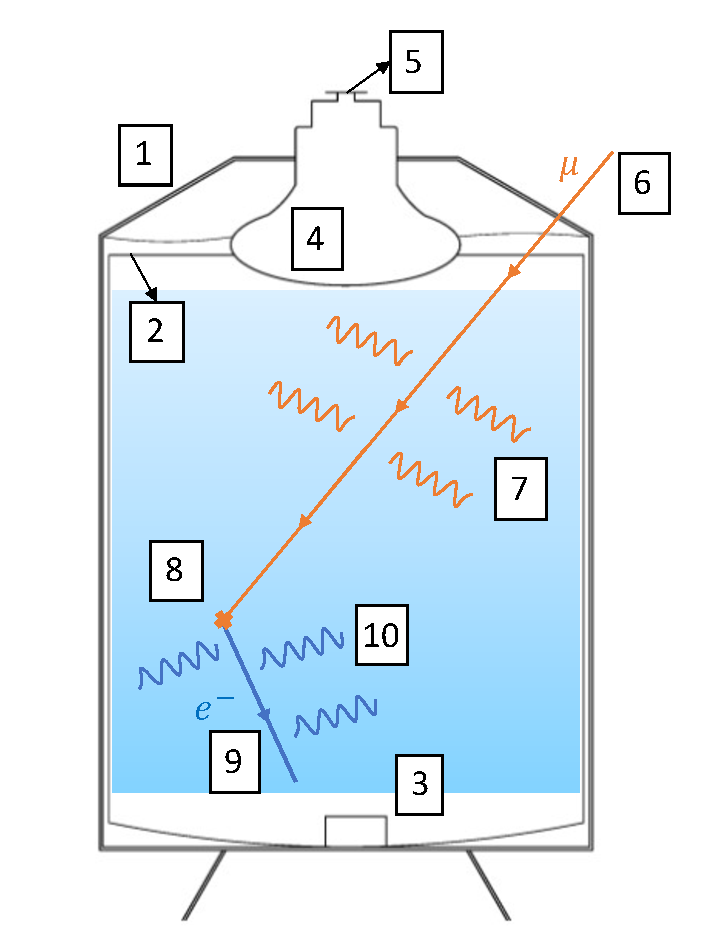
\includegraphics[width=0.6\linewidth]{Figuras/TachoFinal.pdf}
    \caption{Esquema del detector de muones utilizado y los fenómenos estudiados. }
    \label{fig:Detector}
\end{figure}

Por encima del tubo fotomultiplicador se encuentra un circuito de procesamiento de señal diseñado y construido para el proyecto LAGO que acondiciona
la salida del tubo a distintas amplificaciones. La señal de la máxima etapa de amplificación del tubo es transmitida por cable coaxil a una placa
FPGA (Field Programmable Gate Array). Allí, un conversor analógico digital (ADC) de 10 bits realiza una reconstrucción discreta de la señal 
para luego poder ser procesada por computadora. En la misma placa, con un programa de python se detectan picos de voltaje en estas señales digitalizadas 
que indiquen la incidencia de un muón o un decaimiento. Esto se discrimina considerando un valor umbral de voltaje a superar por la señal.  
La morfología de de la señal en el ADC típica de uno de estos picos se exhibe en la Figura \ref{fig:PicoProm}.


\begin{figure} [H]
    \centering
    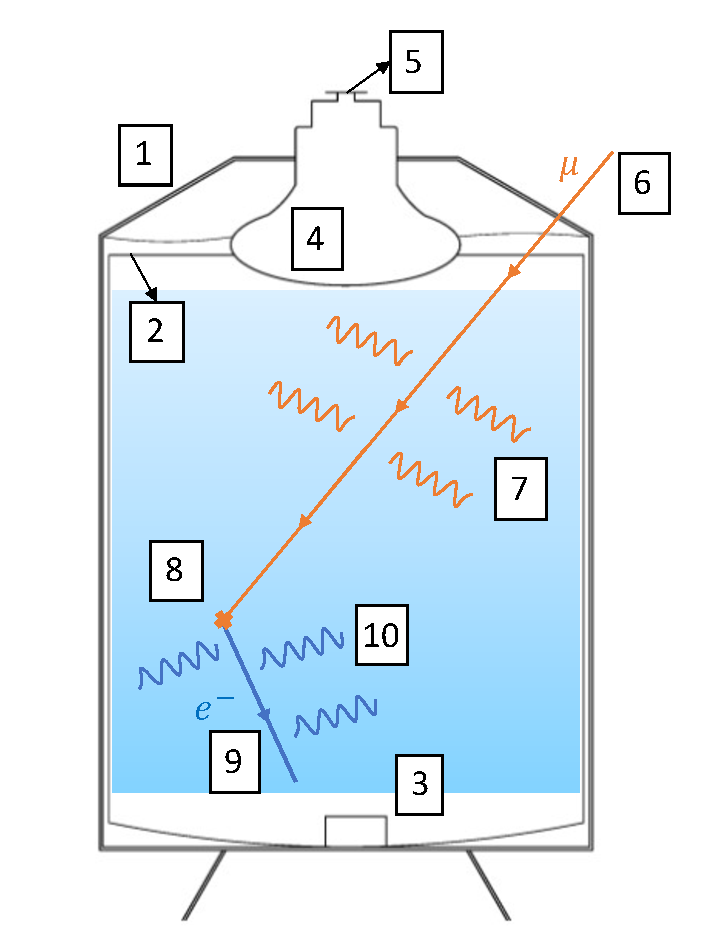
\includegraphics[width=0.6\linewidth]{Figuras/TachoFinal.pdf}
    \caption{Gráfica de una señal típica vista en el ADC debido a incidencias y decaimientos de muones. Este gráfico corresponde a una
            señal extraida aleatoriamente durante el experimento}
    \label{fig:PricoProm}
\end{figure}

En este experimento la placa FPGA utilizada 

\bibliographystyle{unsrt}
\bibliography{referencias}

\end{document}


